\documentclass[a4paper]{extarticle}
\usepackage[utf8]{inputenc}
\usepackage[a4paper, margin=1in]{geometry}

\usepackage{amssymb}
\usepackage{amsmath}
\usepackage{enumitem}
\usepackage{tcolorbox}
\usepackage{fancyhdr}
\usepackage{graphicx}
\usepackage{float}

\setlength{\parindent}{0em}
\setlength{\parskip}{0.4em}

\definecolor{theoremblue}{RGB}{1, 73, 124}
\definecolor{corollaryblue}{RGB}{70, 143, 175}
\definecolor{exampleblue}{RGB}{137, 194, 217}

\newtcolorbox{tbox}{colback=theoremblue!20,colframe=theoremblue,
boxrule=0pt,arc=0pt,boxsep=2pt,left=2pt,right=2pt,leftrule=2pt}

\newtcolorbox{cbox}{colback=corollaryblue!20,colframe=corollaryblue,
boxrule=0pt,arc=0pt,boxsep=2pt,left=2pt,right=2pt,leftrule=2pt}

\newtcolorbox{ebox}{colback=exampleblue!20,colframe=exampleblue,
boxrule=0pt,arc=0pt,boxsep=2pt,left=2pt,right=2pt,leftrule=2pt}

\title{IntroML - Lecture Notes Week 1}
\author{Ruben Schenk, ruben.schenk@inf.ethz.ch}
\date{\today}

\pagestyle{fancy}
\fancyhf{}
\rhead{ruben.schenk@inf.ethz.ch}
\rfoot{Page \thepage}
\lhead{IntroML - Lecture Notes Week 1}

\begin{document}

\maketitle

\section{Examples of Machine Learning Problems}

\begin{ebox}
The \textbf{Machine Learning (ML) approach} for supervised learning is that machines should learn rules using some example data.
\end{ebox}

\subsection{Supervised Learning}

\begin{figure}[H]
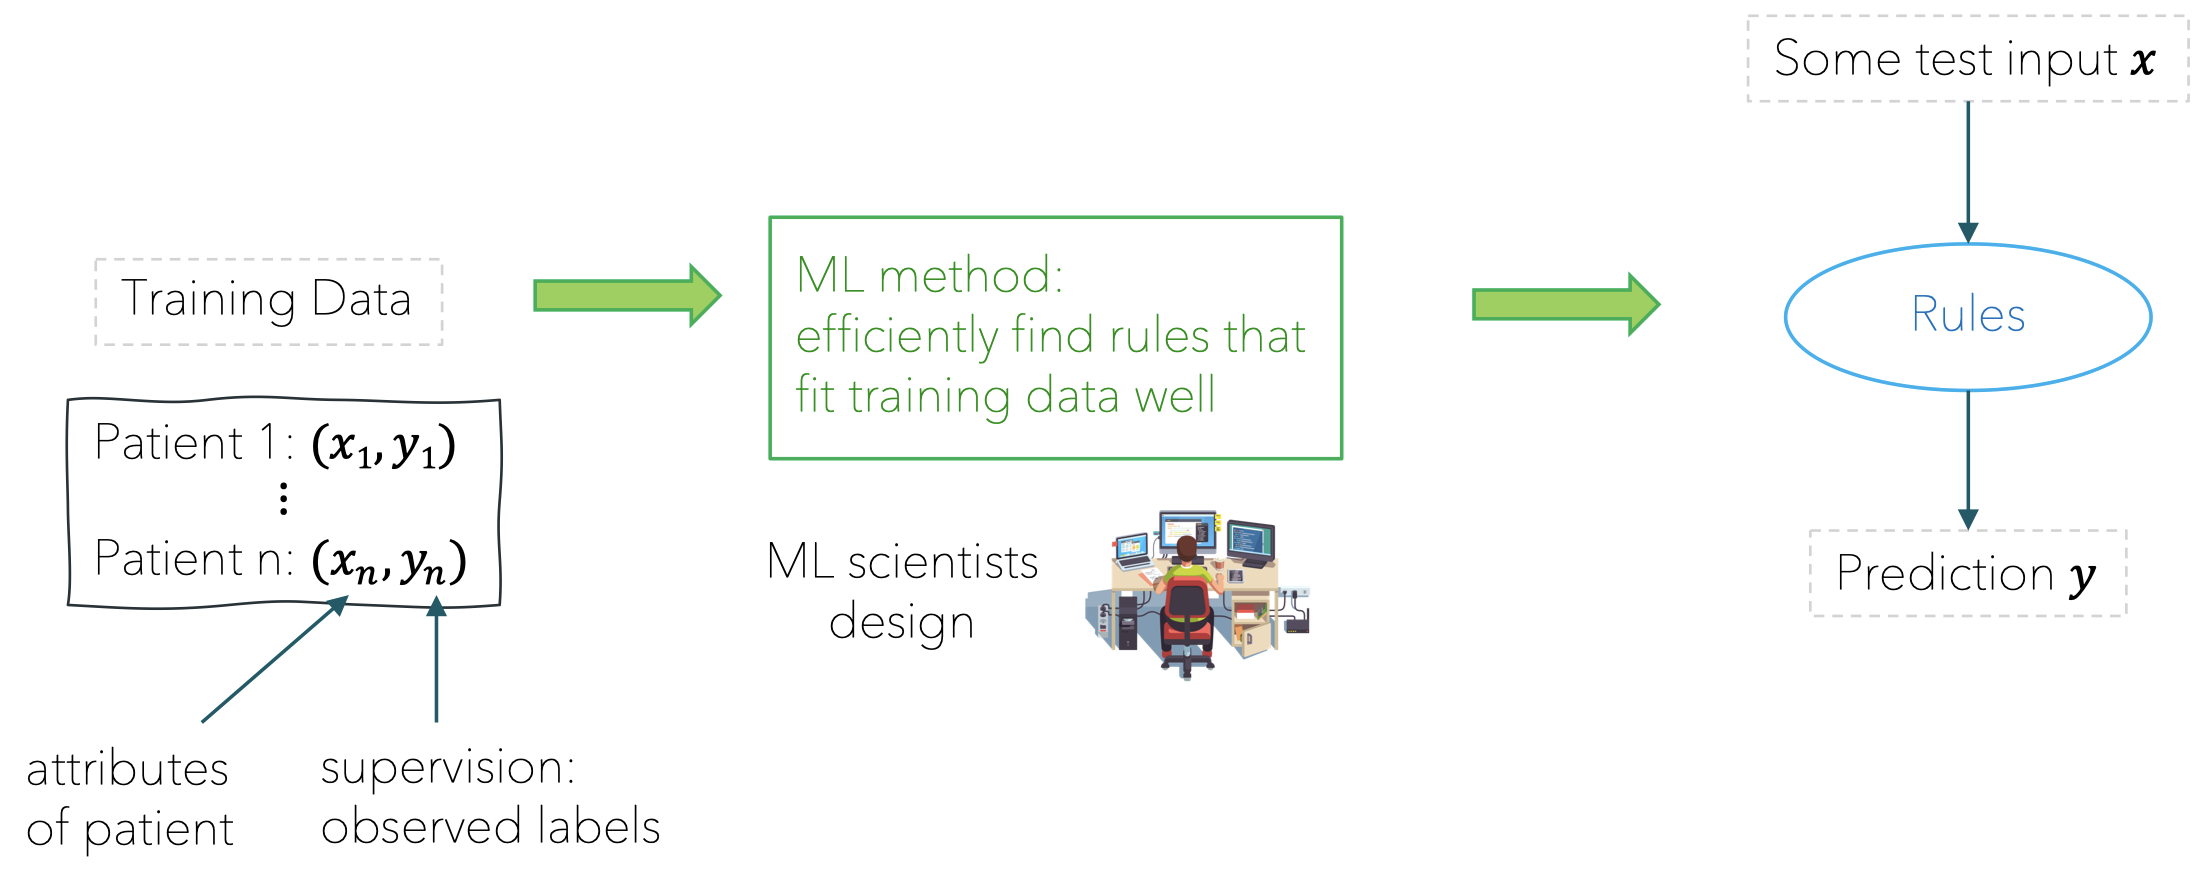
\includegraphics[width=15cm]{../images/IntroML_Fig1-1}
\centering
\end{figure}

The different supervised learning tasks are as follows:

\begin{itemize}
	\item \textit{Classification:} Predict the class (discrete scalar) of an input.
	\item \textit{Regression:} Predict a value (continuous scalar) for an input.
	\item \textit{Structured Prediction:} Predict an output beyond scalars.
\end{itemize}

\subsection{Unsupervised Learning}

\begin{figure}[H]
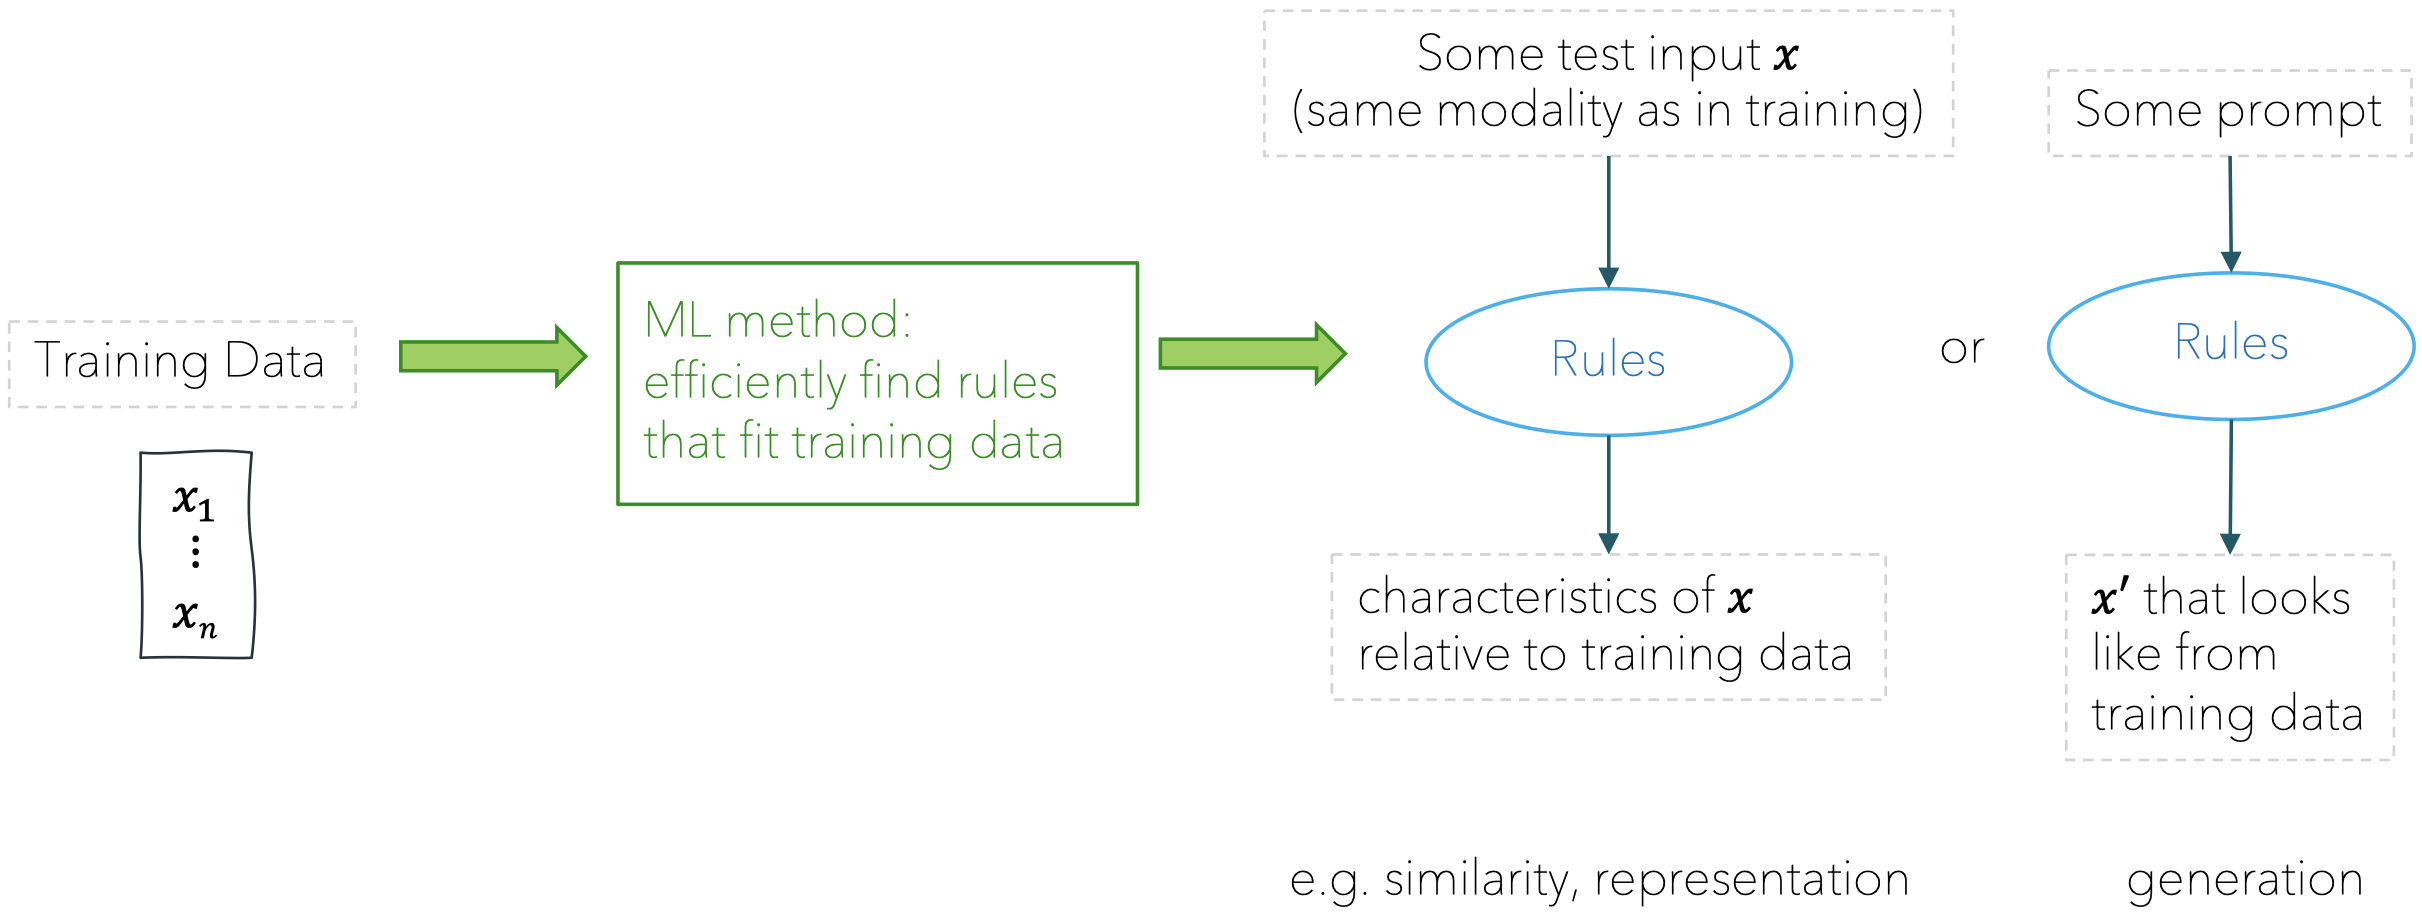
\includegraphics[width=15cm]{../images/IntroML_Fig1-2}
\centering
\end{figure}

Some common goals using unsupervised learning on the characteristics of some data are:

\begin{itemize}
	\item Anomaly detection of "unusual" data points
	\item Identification of (relevant) unobserved variables (such as features and classes)
	\item Compact representation and compression of data sets
	\item Generation of new data
\end{itemize}

Some ML methods to learn characteristics of the data (that are covered in the class) include:

\begin{itemize}
	\item \textit{Clustering,} e.g. for learning similarity and anomaly of points
	\item \textit{Dimensionality reduction,} e.g. for learning compact representations
	\item \textit{Generative modelling,} e.g. for feature learning and data generation
\end{itemize}

\subsection{Machine Learning Pipeline}

We will explore the \textbf{machine learning pipeline} by considering an example where we want to list a house for sale but do not know which price is right. We therefore try to find the average market price for houses of our kind. The ML pipeline consists of the following steps:

\paragraph{Step 0} Find representation for the house

We have to determine how to represent houses in digital fashion, for example using a \textit{vector of attributes.}

\paragraph{Step 1} Collect training data

After we found a digital model of our house, we need to collect the \textit{training data,} i.e. attributes and sales prices from other houses and our own house.

\paragraph{Step 2} Learn

With the attributes of both training data and our own house, we need to efficiently find a function \(\hat{f} \in F\) that fits our training data.

\paragraph{Step 3} Predict

Finally, with our model \(\hat{f}\) and the attributes of our house, we can predict the average price for our house.

\section{Linear Regression}

\subsection{Simple Linear Regression in 1D}

\subsubsection{Introduction}

Coming back to our previous example of selling a house, consider the case where the only attributes are \(x\), the size of the house in \(m^2\), and \(y\), the sales price in CHF.

After applying that data to out ML pipeline, we might end up with a model \(\hat{f}\) as follows:

\begin{figure}[H]
	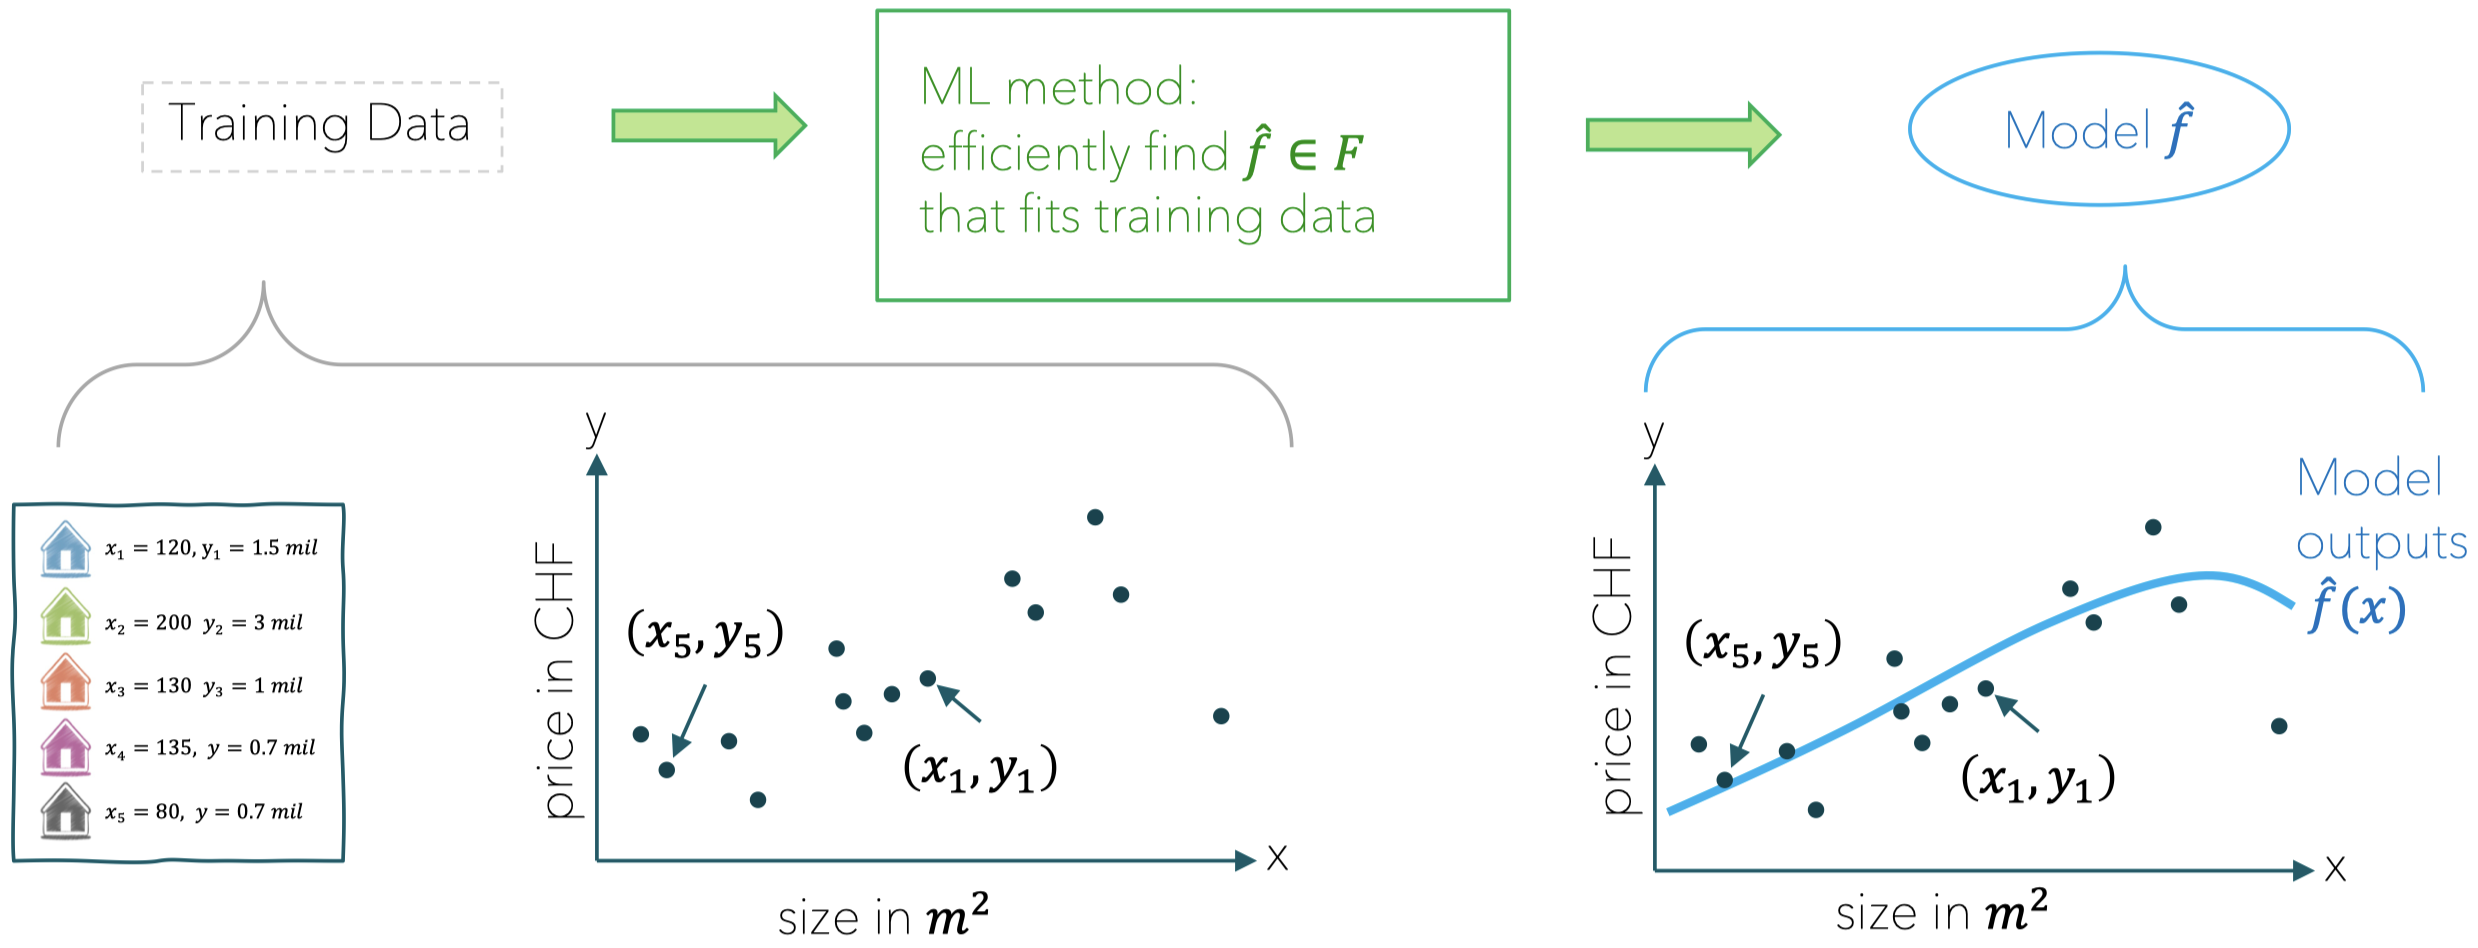
\includegraphics[width = 15cm]{../images/IntroML_Fig1-3}
	\centering
\end{figure}

Finally, with our predict model \(\hat{f}\) and the attributes of our own house, we can predict its average market price.

 The main question to ask here is: How do we find the model \(\hat{f}\)? For this to answer we need to define the following three things:

\begin{itemize}
	\item Function class \(F\)
	\item Training loss
	\item Optimization
\end{itemize}

\subsubsection{Function Classes \(F\)}

We might ask ourselves what kind of functions can we fit in 1D data? Obviously, we can fit constant and linear functions, but more generally speaking we are often looking for polynomials or non-linear functions. For this chapter, we focus on linear functions.

\begin{figure}[H]
	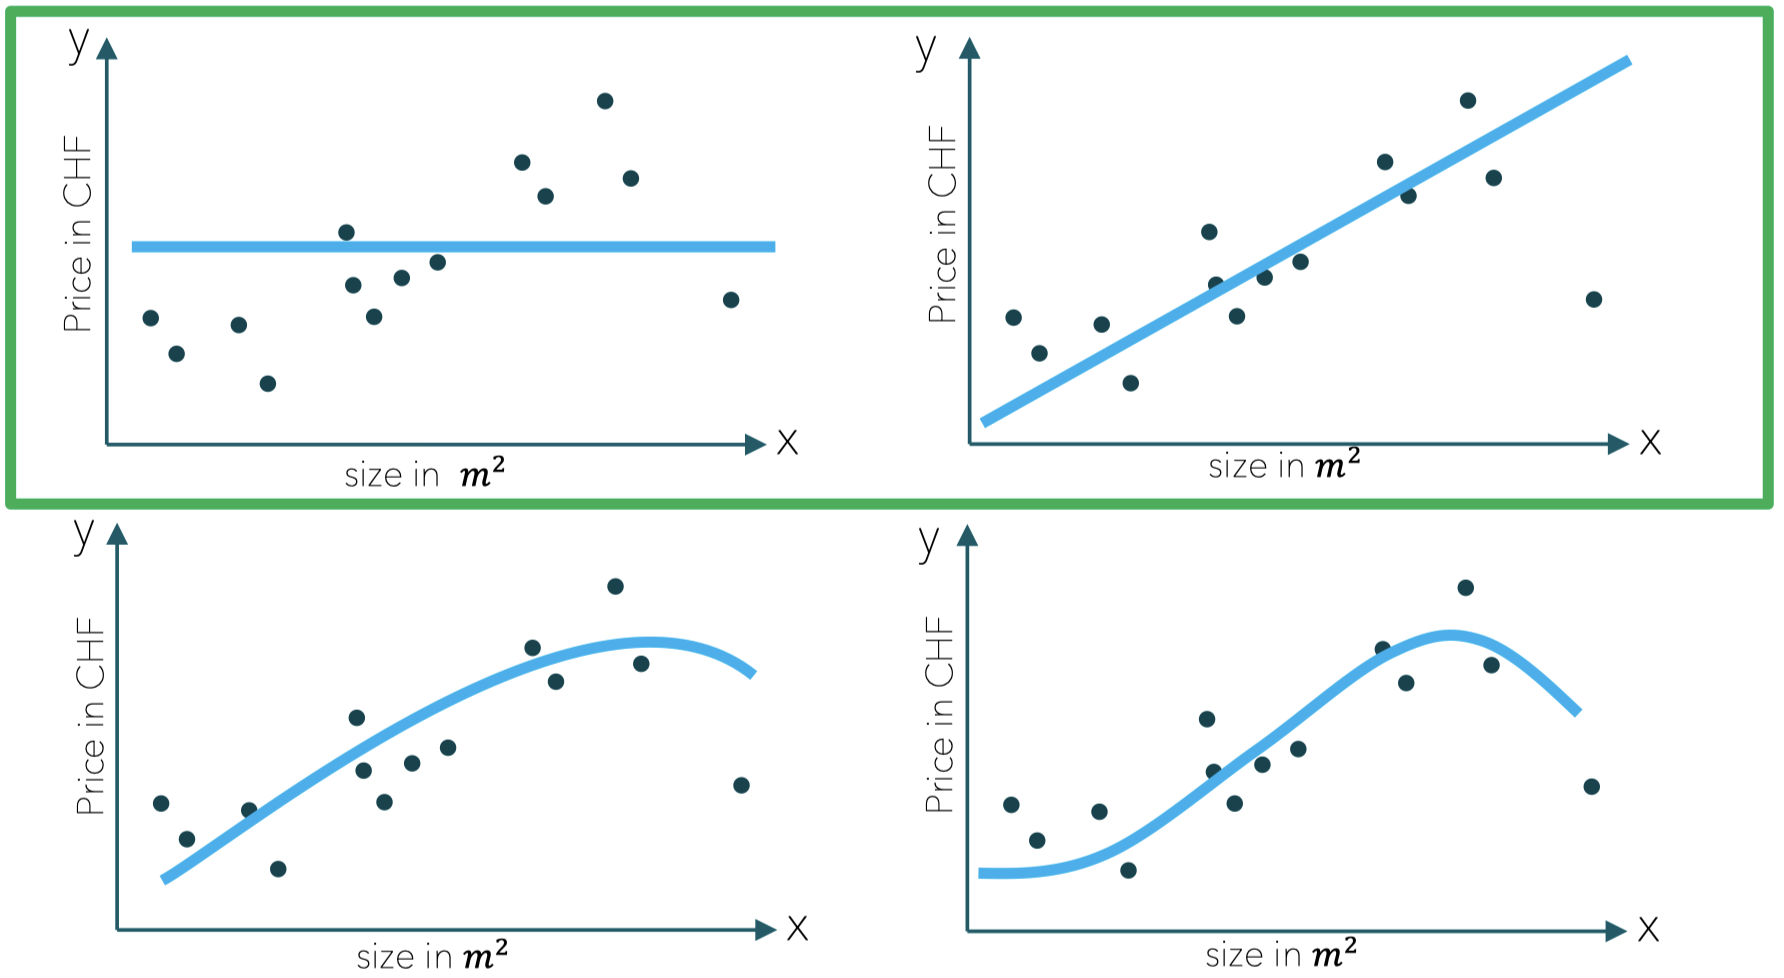
\includegraphics[width = 10cm]{../images/IntroML_Fig1-4}
	\centering
\end{figure}

\subsubsection{Training Losses}

How do we define a \textit{good fit} of the training data? The usual way is if \(f(x)\) is close to \(y\) for most points, that is, if it has a \textbf{low training loss:}

\[
	L(f) = \frac{1}{n} \sum_{i = 1}^n l(f(x_i), \, y_i),
\]

where \(l\) is the \textbf{pointwise loss function,} representing the "closeness" between \(f(x)\) and \(y\) for a point \((x, \, y)\). For our running example, we may choose \((f(x) - y)^2\) as the loss-function (\textbf{squared loss}).

\begin{figure}[H]
	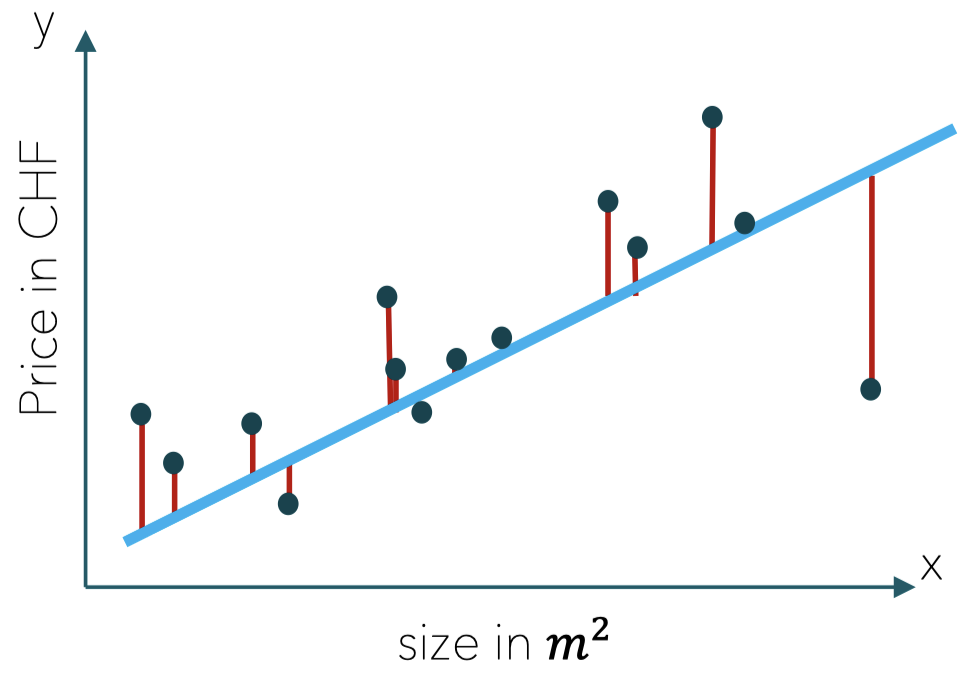
\includegraphics[width = 6cm]{../images/IntroML_Fig1-5}
	\centering
\end{figure}

\subsubsection{Minimizing Squared Loss}

Remember: Our final model is the function \(\hat{f}\) that minimizes the training loss (squared loss on average):

\[
	\hat{f} = \text{argmin}_{f \in F_{Lin}} L(f) = \text{argmin}_{f \in F_{Lin}} \frac{1}{n} \sum_{i = 1}^n (y_i - f(x_i))^2
\]

We call \(\hat{f}\) the \textbf{solution of the ML method linear regression.}

If we recall that all linear functions (\(f(x) = w_0 + w_1x\)) are parameterized by two scalars \(w_0, \, w_1\), searching for a minimum in \(F_{Lin}\) is the same as searching for scalars \(w_0, \, w_1\) that minimize:

\[
	\hat{w} := (\hat{w_0}, \, \hat{w_1}) = \text{argmin}_{w_0,w_1 \in \mathbb{R}} L(w_0, \, w_1) = \text{argmin}_{w_0,w_1 \in \mathbb{R}} \frac{1}{n} \sum_{i = 1}^n (y_i - w_0 - w_1x_i)^2
\]

For simplification, we first fix \(w_0 = 0\), and only optimize \(L(0, \, w_1)\) over \(w_1 \in \mathbb{R}\).

\begin{figure}[H]
	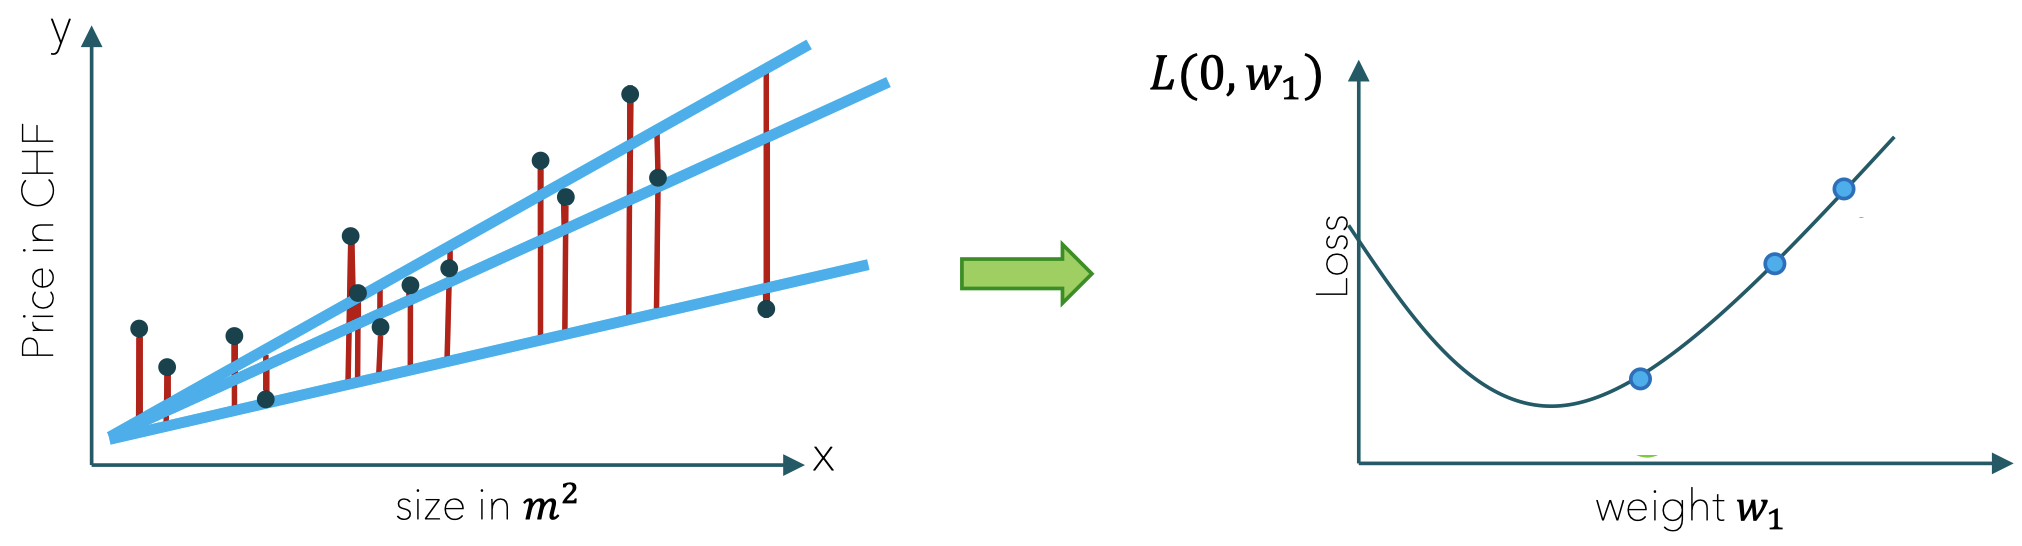
\includegraphics[width = 15cm]{../images/IntroML_Fig1-6}
	\centering
\end{figure}

Since \(L(0, \, w_1) = \frac{1}{n} \sum_{i = 1}^n (y_i - w_1x_i)^2\) is a 1D-quadratic, there's only one minimum where \(L'(0, \, \hat{w}_1) = 0\).

Now we get back to our original problem. More generally, let \(w_0\) again be a variable, i.e. we want to find \(\hat{w} = (\hat{w}_0, \, \hat{w}_1) = \text{argmin}_{w_0,w_1 \in \mathbb{R}} L(w_0, \, w_1)\). Consider the following theorem:

\begin{tbox}
	\textbf{Theorem 2.3 (Necessary Condition for Local Optimality):} Let \(\Omega \subseteq \mathbb{R}^n\) be open and \(f : \Omega \to \mathbb{R}\) a continuously differentiable function. If \(x_0 \in \Omega\) is a local minimizer, then

	\[
		\nabla f(x_0) = 0.	
	\]

	Therefore, when searching for local/global minima, we only have to search within the set of \textit{critical (or stationary) points} defined as \(\{x \in \Omega \, | \, \nabla f(x) = 0\}\).
\end{tbox}

Following this we can conclude, that a global minimum \(\hat{w}\) must satisfy \(\nabla_w L(\hat{w}) = 0\). Hence, the minimum \(\hat{w} = (\hat{w}_0, \, \hat{w}_1)\) satisfies:

\[
	\nabla_w L(\hat{w}_0, \, \hat{w}_1) =
	\begin{pmatrix}
		- \frac{2}{n} \sum_{i = 1}^n (y_i - \hat{w}_0 - \hat{w}_1x_i) \\
		- \frac{2}{n} \sum_{i = 1}^n (y_i - \hat{w}_0 - \hat{w}_1x_i)x_i
	\end{pmatrix}
	= 0
\]

How many minima \(\hat{w}\) are there? It depends on \(\{(x_i, \, y_i)\}_{i = 1}^n\).

\subsubsection{Other Losses}

For now, we have only considered the \textbf{squared loss} as a loss function for our model. Squared loss weighs over- and underestimation the same, and the cost grows quadratically (\textit{large errors hugely penalized}). Instead, one might want:

\begin{itemize}
	\item Ignore outliers (ones with very large penalty) \(\rightarrow\) \textit{Huber loss}
	\item Weigh over- and underestimation differently \(\rightarrow\) \textit{Asymmetric losses}
\end{itemize}

\subsection{Multiple Regression}

\subsubsection{Introduction}

We now consider the case where we have more inputs available. We come back to our selling-a-house example and collect more data of the other houses on the market. For example:

\begin{itemize}
	\item \(x_{[1]}\) = size in \(m^2\)
	\item \(x_{[2]}\) = number of bathrooms
	\item \(x_{[3]}\) = distance to the nearest train station
	\item \(x_{[4]}\) = years since construction
\end{itemize}

This gives us an \textbf{attribute vector} \(x = (x_{[1]}),..., \, x_{[d]}\) and our model of a house is, for example, \(x_1 = (120, \, 2, \, 0.5, \, 1), \, y_1 = 1.5mio\).

\begin{ebox}
	\textbf{Remark:} It is of great importance to not confuse the following two notations:

	\begin{itemize}
		\item \(x_i \rightarrow\) input attributes of sample \(i\)
		\item \(x_{[i]} \rightarrow i\)-th attribute
	\end{itemize}
\end{ebox}

The following visualization shows the ML pipeline for \(d = 2\), however it holds (and especially the upcoming formulas) for any \(d > 1\):

\begin{figure}[H]
	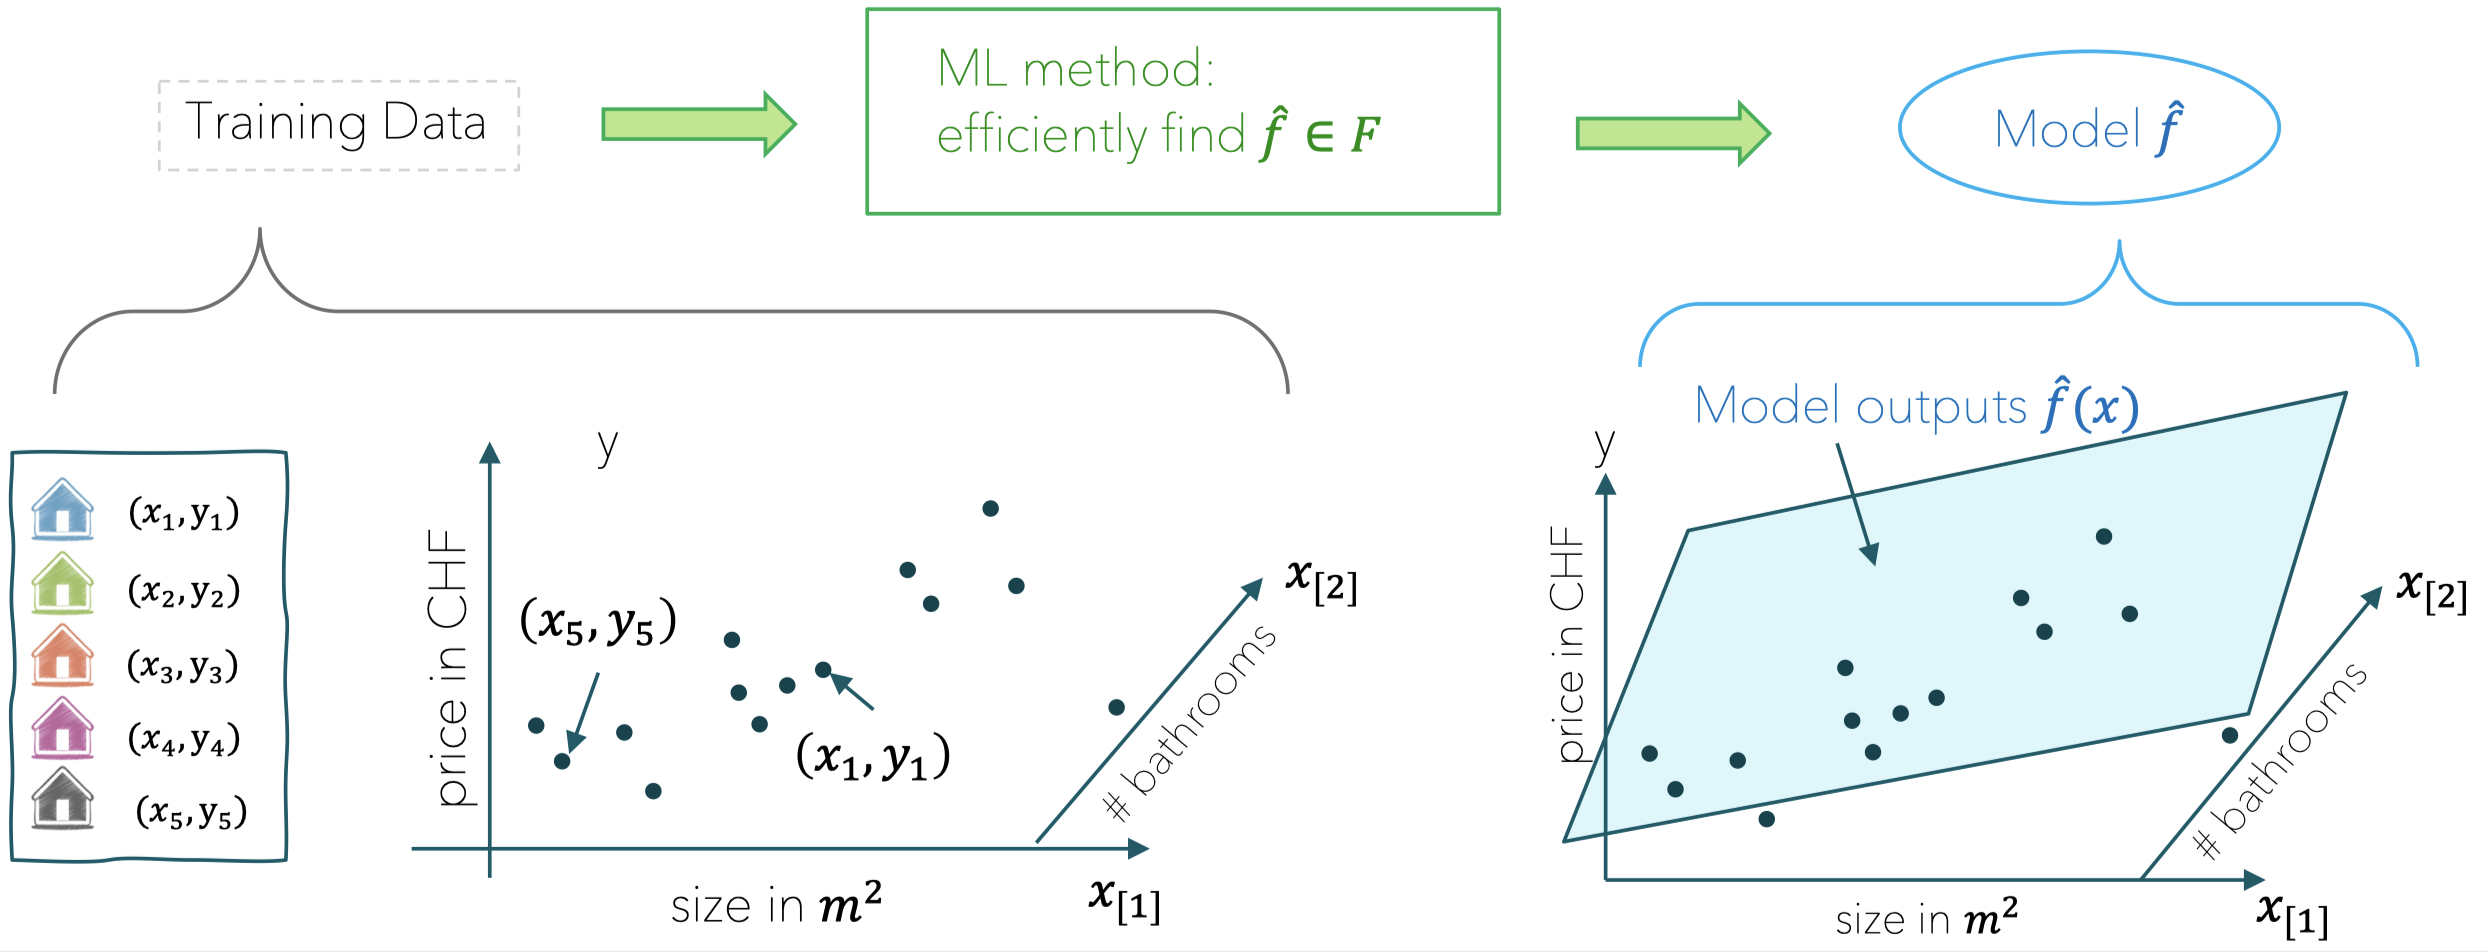
\includegraphics[width = 15cm]{../images/IntroML_Fig1-7}
	\centering
\end{figure}

\subsubsection{Function Classes \(F\)}

The class of linear functions with \(d\) \textit{linear features} is given by:

\[
	F_{Lin} = \{f : f(x) = w_0 + \sum_{j = 1}^d w_jx_{[j]} = w_0 + w^Tx \text{ for } w = (w_1,..., \, w_d) \in \mathbb{R}\}	
\]

For \(d = 2\) this equates to \(f(x) = w_0 + w_1x_{[1]} + w_2x_{[2]}\).

\subsubsection{Training Loss}

Analogous to the 1D-model, the learned model \(\hat{f}\) minimizes the training loss, i.e.:

\[
	\hat{f} = \text{argmin}_{f \in F_{Lin}} L(f) = \text{argmin}_{f \in F_{Lin}} \frac{1}{n} \sum_{i = 1}^n (y_i - f(x_i))^2	
\]

Since \(\hat{f} \in F_{Lin}\) must be of the form \(\hat{f}(x) = \hat{w}_0 + \hat{w}^Tx\), it is equivalent to minimizing over vector \(w\) and scalar \(w_0\):

\[
	\hat{w} = \text{argmin}_{w_0 \in \mathbb{R}, \, w \in \mathbb{R}^d} L(w_0, \, w) = \text{argmin}_{w_0 \in \mathbb{R}, \, w \in \mathbb{R}^d} \frac{1}{n} \sum_{i = 1}^n (y_i - w_0 - w^Tx_i)^2
\]

We can rewrite the training loss \(L\) into \textbf{vector notation:}

\[
	L(w_0, \, w) = \frac{1}{n} \sum_{i = 1}^n (y_i - w_0 - w^Tx_i)^2 = \frac{1}{n}||y - \textbf{1}w_0 - Xw||^2,
\]

where \(\textbf{1} = (1,..., \, 1) \in \mathbb{R}^n\) is the all-ones vector.

\subsubsection{Minimizing Training Loss}

Again, for simplicity, let's set \(w_0 = 0\) and minimize over \(w\). Plugging that into \(L(w_0, \, w) = \frac{1}{n}||y - \textbf{1}w_0 - Xw||^2\) yields:

\[
	L(0, \, w) = \frac{1}{n}||y - Xw||^2 = \frac{1}{n}||y||^2 - \frac{2}{n}y^TXw + \frac{1}{n}w^TX^TXw,
\]

with gradient \(\nabla_w L(0, \, w) = \frac{2}{n}(X^TXw - X^Ty)\) and Hessian \(D^2L(0, \, w) = \frac{2}{n}X^TX\).

We now look at two ways to find the minimum:

\begin{itemize}
	\item Stationary point condition (gradient = \(0\))
	\item Geometric argument (orthogonal projection)
\end{itemize}

\paragraph{Stationary Point Condition}

Again, the minimum \(\hat{w} = \text{argmin}_w L(0, \, w)\) must be a stationary point, i.e. satisfying \(\nabla_w L(0, \, \hat{w}) = 0\). All stationary points of this quadratic loss \(\frac{1}{n}||y-Xw||^2\) are minima, because the Hessian \(\frac{2}{n}X^TX\) is positive-definite.

\(\nabla_w L(0, \, w) = \frac{2}{n}(X^TXw - X^Ty)\) together with stationary point condition \(\nabla_w L(0, \, \hat{w}) = 0\) yields:

\begin{tbox}
	\[
		X^Ty = X^TX\hat{w} \Rightarrow \hat{w} = (X^TX)^{-1}X^Ty
	\]
\end{tbox}

\paragraph{Geometric Argument}

Since the set of all possible \(Xw\) is given by \(\text{span}(w)\), the closest point to \(y\) on \(\text{span}(X)\) is the orthogonal projection of \(y\) onto \(\text{span}(X)\). We denote this projection as \(\Pi_Xy\).

\begin{figure}[H]
	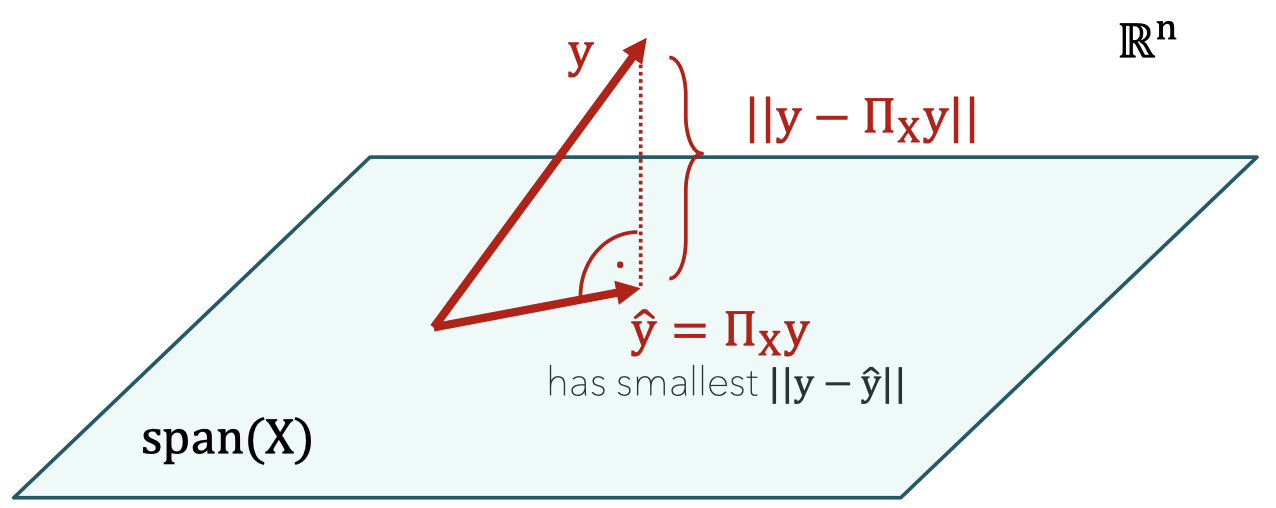
\includegraphics[width = 6cm]{../images/IntroML_Fig1-8}
	\centering
\end{figure}

We now need to derive the equation for the vector \(\hat{w}\) such that \(X\hat{w} = \Pi_Xy\). Since the residual \(y - X\hat{w}\) is orthogonal to all vectors \(v \in \text{span}(X)\), we have that \((y - X\hat{w})^TXw = 0\) for all \(w \in \mathbb{R}^d\). Hence, we require \(X^T(y-X\hat{w}) = 0 \Leftrightarrow X^Ty = X^X\hat{w}\) (also called \textbf{normal equations}).

Finally, this yields again the unique solution \(\hat{w} = (X^TX)^{-1}X^Ty\) if \(X^TX\) is invertible.

\end{document}